\chapter{ Utility Battery Energy Storage - Energy Arbitrage Only}
In the most elementary form, energy arbitrage entails charging when the wholesale spot price is low, and discharging when the wholesale price is high. Whilst conceptually simple, the purchase price of a battery is high, and there are physical limitations on charge/discharge and the frequency of high spot prices is relatively infrequent.
\section{ Algorithm and Software Selection }
\parencite{McConnell} used COIN-OR Linear Program solver to find the optimal dispatch for a battery performing energy arbitrage. Linear programming is one of the most common optimisation techniques. Leonard Kantrovich was awarded the 1975 Nobel Price in Economics for the optimal allocation of resources using linear programming \parencite{PythonPulp}. Examples of problems that can be solved by linear programming include:
\begin{itemize}
    \item Scheduling – Rota or Factory scheduling to meet production/workload demands at lowest cost
    \item Resourcing Problems – How best to allocate resources to maximise profits
    \item Sudoku
\end{itemize}
PuLP is a suitable tool to perform LP in this thesis for the following reasons: 
\begin{itemize}
    \item Library for Python which is a highly supported coding language with an emphasis on rapid development, clarity of code and a simple object model. 
    \item PuLP works entirely within the syntax of Python and represents optimisation problems and decision variables in  a way that is very similar to the original mathematical expression. 
    \item PuLP is available under a permissive open-source license that encourages and facilitates the use of PuLP inside other projects that need linear optimisation capabilities.
\end{itemize}
\section{ Methodology }
The following algorithm represents the methodology for optimising energy arbitrate in a deterministic model with perfect foresight of energy prices over the optimisation window.
\begin{align*}
  \max \sum_{i=0}^T \left(x^{(i)}_c + x^{(i)}_d \right) p^{(i)} \times \left( \frac{l}{60} \right)
\end{align*}
Subject to the constraints:
\begin{alignat} {2}
    -P_{max} &\leq x^{(i)}_c \leq 0  &&\forall i \in [0,T]\\
    0 &\leq x^{(i)}_d \leq P_{max}  &&\forall i \in [0,T]\\
    0 &\leq E^{(i)} \leq E_{max} &&\forall i \in [0,T] \\
    E^{(0)} &= E_{\text{init}} - \left(x^{(0)}_c \eta_c + x^{(0)}_d \frac{1}{\eta_d} \right) \frac{l}{60} && \\
    E^{(i)} &= E^{(i-1)} - \left(x^{(i)}_c \eta_c + x^{(i)}_d \frac{1}{\eta_d} \right) \frac{l}{60} \hspace{1cm} &&\forall i \in [1,T] 
\end{alignat}
Where,
{\renewcommand{\arraystretch}{2}}
\begin{center}
    \begin{tabular}{p{0.8cm} p{5.5cm} p{0.8cm} p{5.5cm}}
    \textbf{Constants} & & \textbf{Variables} & \\
    $P_{max}$ & Power Capacity of BESS (MW) & $x^{(i)}_c$ & Charge power at time $i$ (MW)   \\ 
    $E_{max}$ & Storage Capacity of BESS (MWh) & $x^{(i)}_c$&  Discharge power at time $i$ (MW)  \\
    $E_{\text{init}}$ & Initial Storage Level of BESS (MWh)& $E^{(i)}$ &Storage level at time $i$ (MWh)\\
    $l$ & length of time interval in minutes & & \\
    $\eta_c$ & Charge efficiency (\%) & &\\
    $\eta_d$ & Discharge efficiency (\%) & &\\
    $p^{(i)}$ &  Energy price at time $i$ (\$/MWh) & &\\
    $T$ &  Total number of time intervals & &\\
    \end{tabular}
\end{center}
To implement this algorithm, the following methodology was undertaken;
\begin{enumerate}
    \item Configure a Python 3.7 environment.
    \item Import price data via NEMOSIS:  \url{https://github.com/UNSW-CEEM/NEMOSIS}. NEMOSIS is a simple tool for creating datasets using publicly available information about the Australian National Electricity Market (NEM).
    \item Create a battery object.
    \item PuLP python optimisation problem formulation;
    \begin{enumerate}
        \item Identify the Decision Variables
        \item Formulate the Objective Function using the decision variables
        \item Formulate the Constraints
    \end{enumerate}
\end{enumerate}
It is crucial to note that the energy arbitrage only model assumes the battery is a price-taker,and has perfect foresight of price.
\section{ Analysis }
\subsection{ Method Validation }
As shown in Figure \ref{fig:simple_output}, the dispatch logic charging during low prices, and discharging during high prices is effective. Note in Figure \ref{fig:simple_output} a single trip efficiency of 90\% or round trip efficiency of 81\% is implemented. This is a conservative measure, with Tesla stating their Power Pack round trip efficiency is 88\% \url{https://www.tesla.com/en_AU/powerpack}. 
\begin{figure}[H]
    \centering
    \makebox[\textwidth][c]{    \includegraphics[width=1.1\textwidth]{"Pictures/Chapter3/battery_plot".pdf}}
    \caption{BESS Output - 2018-01-01}
    \label{fig:simple_output}
\end{figure}
In order to validate the model, \parencite{Wang} provides energy arbitrage revenues for a 1MW ESS with capacity between 1-8MWh, using NEM price data for years 2010-2013 with perfect foresight. The model assumes 90\% single trip efficiency. The findings are summarised in Figure \ref{fig:wang_ea}. 
\begin{figure}[H]
    \centering
    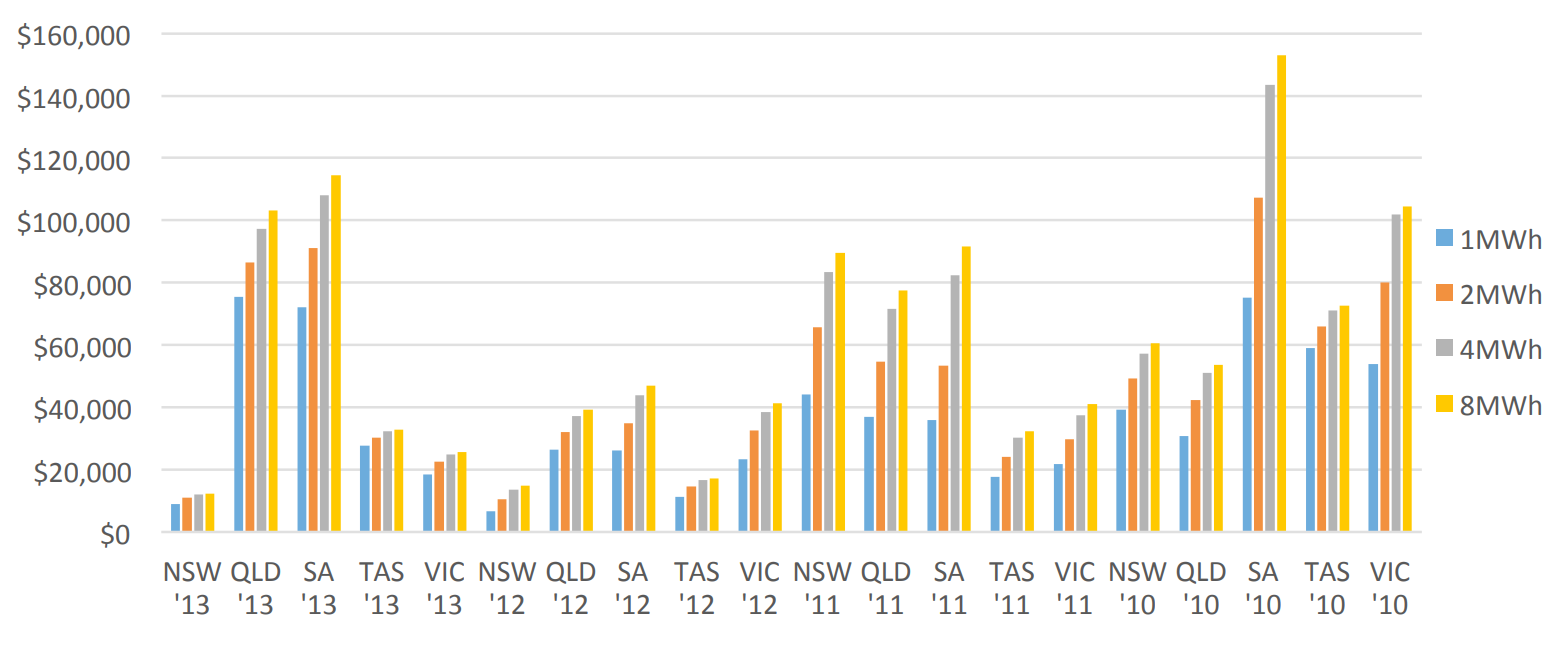
\includegraphics{Pictures/Chapter3/wang_ea.PNG}
    \caption{Energy Arbitrage - Geographic and Temporal Comparison (Wang 2016)}
    \label{fig:wang_ea}
\end{figure}
Below, Figure \ref{fig:wang_ea_comparion} is the implementation of the python model replicating Wang's results. 
\begin{figure}[H]
    \centering
    \makebox[\textwidth][c]{    \includegraphics[width=1\textwidth]{"Pictures/Chapter3/ae_wang_comparison".pdf}}
    \caption{Energy arbitrage annual revenue for a 1 MW / 1 MWh BESS by region 2010 - 2013}
    \label{fig:wang_ea_comparion}
\end{figure}
\begin{wrapfigure}{r}{0.6\textwidth}
    \begin{center}
        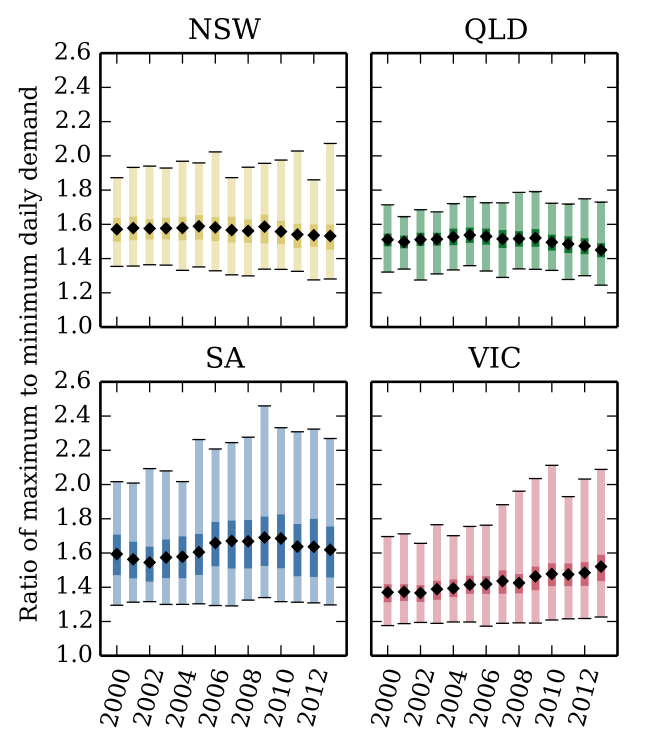
\includegraphics[width=0.4\textwidth]{Pictures/Chapter3/energy_vol.png}
    \end{center}
    
    \caption{National Electricity Market Demand Volatility \parencite{McConnell}}
    \label{fig:demand_volatility}
\end{wrapfigure}
Given Figures \ref{fig:wang_ea} and \ref{fig:wang_ea_comparion} exhibit identical characteristics, this validates the energy only model. This preliminary example also highlights a number of key findings;
\begin{enumerate}
    \item NSW is on average the worst performing state for energy arbitrage.
    \item SA is consistently a high performer relative to other states.
    \item Large discrepancies can occur year-to-year.
    \item Additional storage which increases the cost of a battery proportionally offers diminishing returns for all example. This indicates that short price spikes generally drive revenue, rather than sustained high prices periods. 
\end{enumerate}
Figure \ref{fig:demand_volatility} provided by \textcite{McConnell} highlights the daily variation in demand for each NEM jurisdiction (excl. TAS). Demand volatility which inherently drives price volatility, generally reflects economic and climatic factors. As shown in Figure \ref{fig:demand_volatility}, South Australia has the highest ratio of maximum to minimum daily demand.  
\subsection{ Dependency on Price Dynamics }
Figure \ref{fig:revenue_duration} displays a revenue duration curve of a 1MW/1MWh BESS with 90\% round-trip efficiency from FY 2010 - 2017. The logarithmic scale clearly indicates that less than 10\% of the time, a very significant proportion of revenue is raised from infrequent, high price events. Figure \ref{fig:revenue_duration} also demonstrates an increase in overall BESS revenue - beyond 2013 (not reflected in Figure \ref{fig:wang_ea_comparion}). 
\begin{figure}[H]
    \centering
    \makebox[\textwidth][c]{    \includegraphics[width=1\textwidth]{"Pictures/Chapter3/Revenue Duration Curve for FY10 - FY17".pdf}}
    \caption{Revenue Duration Curve for FY10 - FY17}
    \label{fig:revenue_duration}
\end{figure}
\begin{wrapfigure}{r}{0.6\textwidth}
    \begin{center}
        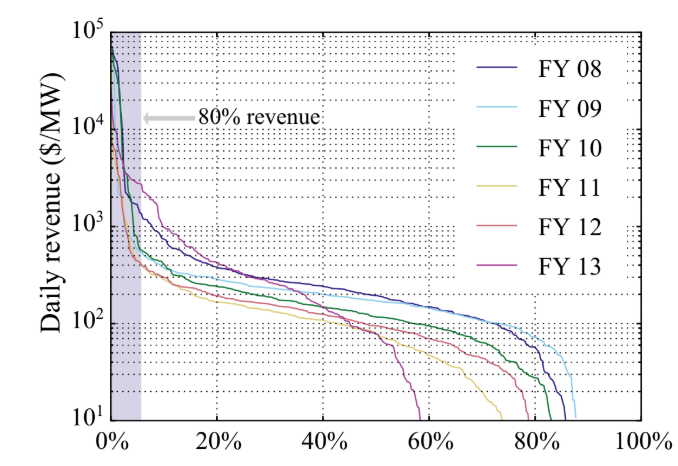
\includegraphics[width=0.6\textwidth]{Pictures/Chapter3/mcconnell_revenue_duration.png}
    \end{center}
    \caption{BESS Revenue Duration Curve (McConnell 2014)}
    \label{fig:mcconnell_rev_duration}
\end{wrapfigure}
 Again, the work of McConnell reinforces this notion in Figure  \ref{fig:mcconnell_rev_duration}. Overall, this phenomenon is expected due to the high Market Clearing Price (MCP) of the NEM at \$14,500.  A high MCP is an essential ingredient to electricity market design. In case of scarcity situations and extreme market fundamentals – such as a heat wave in South Australia, prices may sore to \$14,500/MWh for a number of intervals. This might sound extreme, but have been observed from time to time in the past few years. Such economically justified scarcity prices have a negligible impact on the average price of
electricity for end consumers – however, they are vital for the profitability of flexible power plants \parencite{scarcity_pricing}. 
\subsection{ Seasonal Impact }
Figure \ref{fig:mcconnell_heatmap} illustrates the average optimal operating regime for different hours of the day and different days of the year in South Australia. As expected, the dispatch follows the seasonal price and demand patterns characterised by a bi-modal peak in winter and an afternoon peak in summer.
\begin{figure}[H]
    \centering
    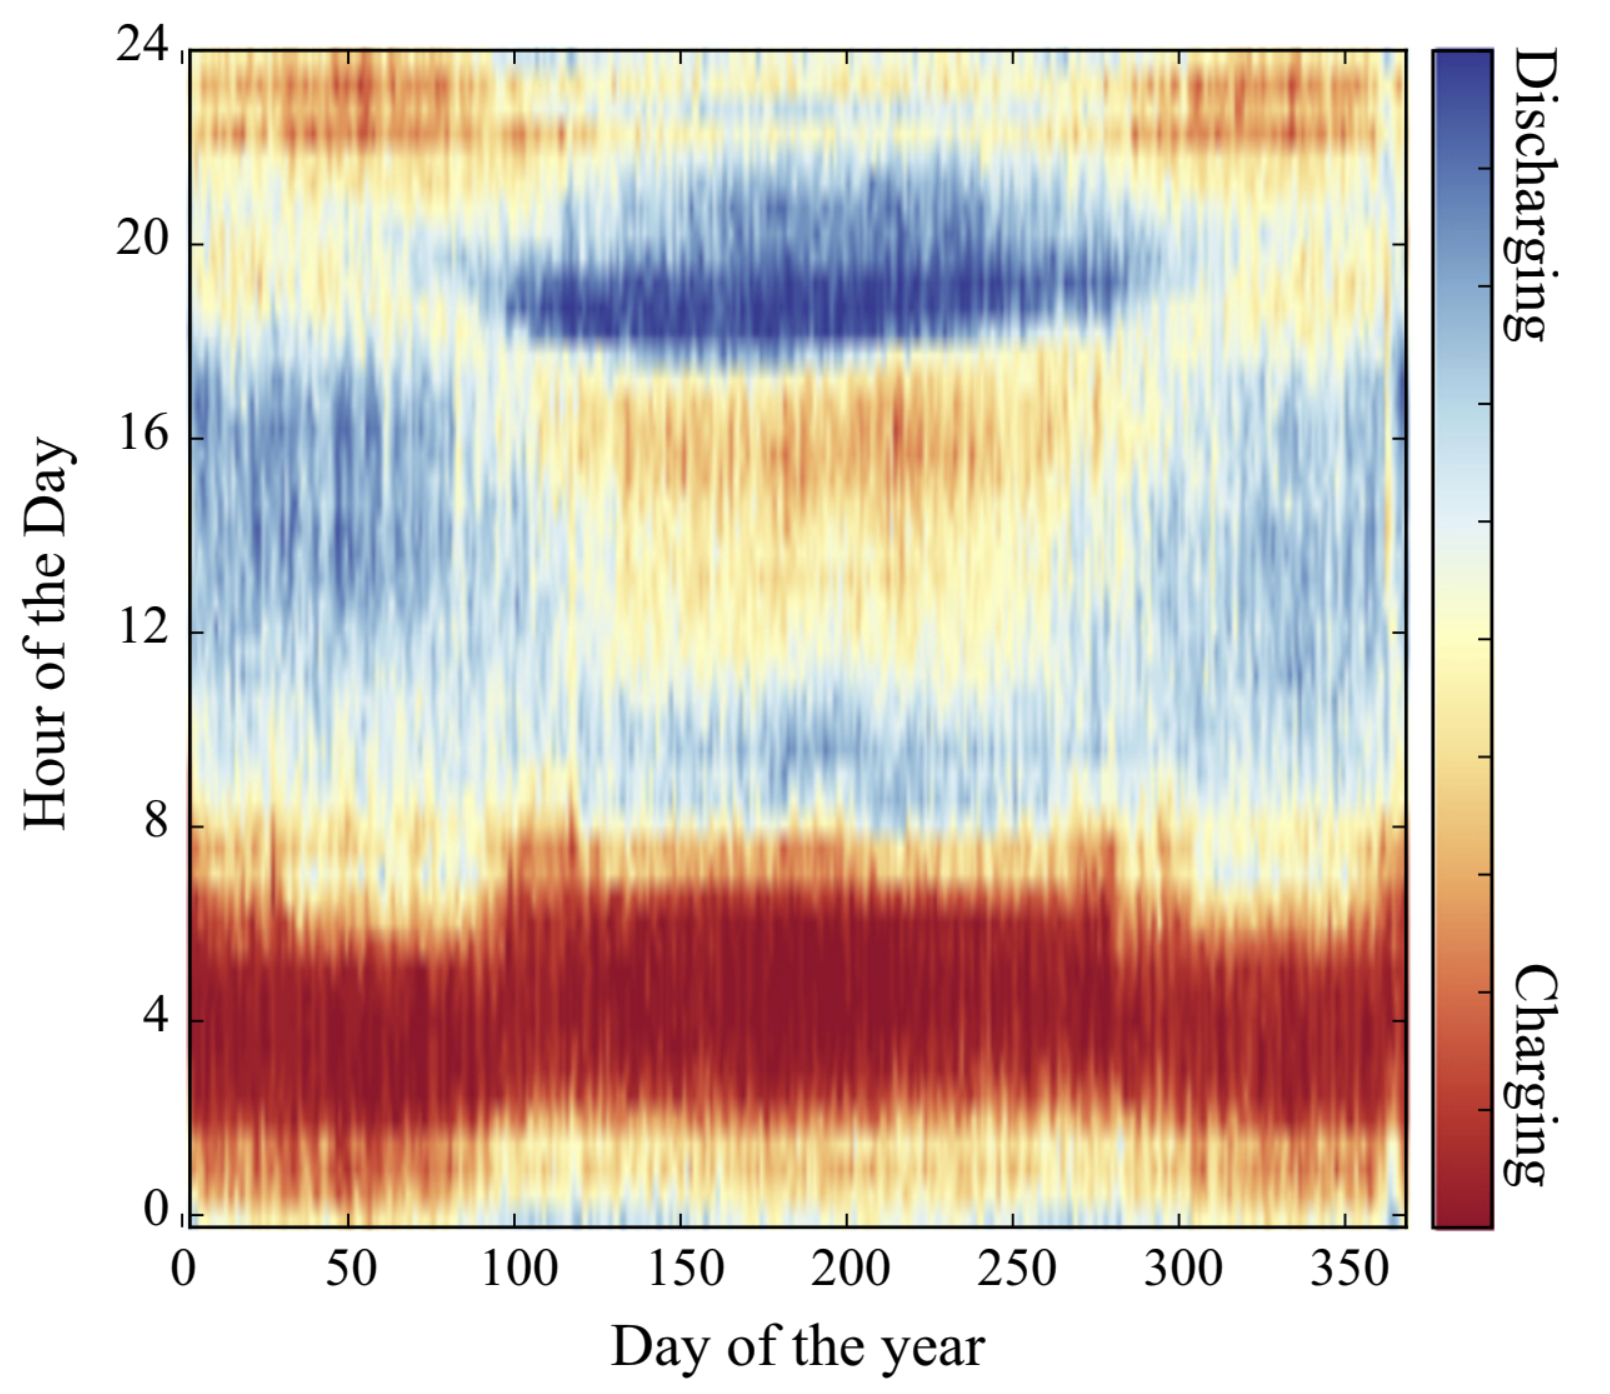
\includegraphics[width=0.6\textwidth]{Pictures/Chapter3/mcconnel_heatmap.png}
    \caption{Optimal BESS operation characteristics, for winter and summer months of the year. (McConnell, 2015)}
    \label{fig:mcconnell_heatmap}
\end{figure}
Figure \ref{fig:heatmap} extends the analysis of McConnell, demonstrating the impact that storage capacity has on operating characteristics. The contrast in both sides of the subplot is that 1 Hour storage often has idle times (cream colour) whilst 8 Hours of storage is constantly either charging or discharging.
\begin{figure}[H]
    \centering
    \makebox[\textwidth][c]{    \includegraphics[width=1\textwidth]{"Pictures/Chapter3/South Australia - 2017".pdf}}
    \caption{Optimal BESS operation characteristics, for winter and summer months of the year, varying storage capacity.}
    \label{fig:heatmap}
\end{figure}
\subsection{ Impact of Throughput Constraints }
Below Figure \ref{fig:throughput_limit} shows the impact of applying a 365 cycles per annum throughput limit on a battery energy storage system. As shown, for both region and storage capacity - throughput limitations typically don't hinder arbitrage revenues significantly. 
\begin{figure}[H]
    \centering
    \makebox[\textwidth][c]{    \includegraphics[width=1\textwidth]{"Pictures/Chapter3/Impact of Throughput on Annual Revenue_ 1 MW Battery".pdf}}
    \caption{Impact of Throughput on Annual Revenue: 1 MW Battery}
    \label{fig:throughput_limit}
\end{figure}
\subsection{ Recent Trends and Driving Factors for Energy Arbitrage Revenue }
Figure \ref{fig:wang_plot_full} extends Figure \ref{fig:wang_ea_comparion} and shows the energy arbitrage revenue with perfect foresight, for a 1MW BESS including the calendar years (15,16,17,18). 
\begin{figure}[H]
    \centering
    \makebox[\textwidth][c]{    \includegraphics[width=1\textwidth]{"Pictures/Chapter3/Energy Arbitrage - Geographic and Temporal Comparison".pdf}}
    \caption{Energy arbitrage annual revenue for a 1 MW / 1 MWh BESS by region 2010 - 2018}
    \label{fig:wang_plot_full}
\end{figure}
\begin{wrapfigure}{r}{0.6\textwidth}
    \begin{center}
        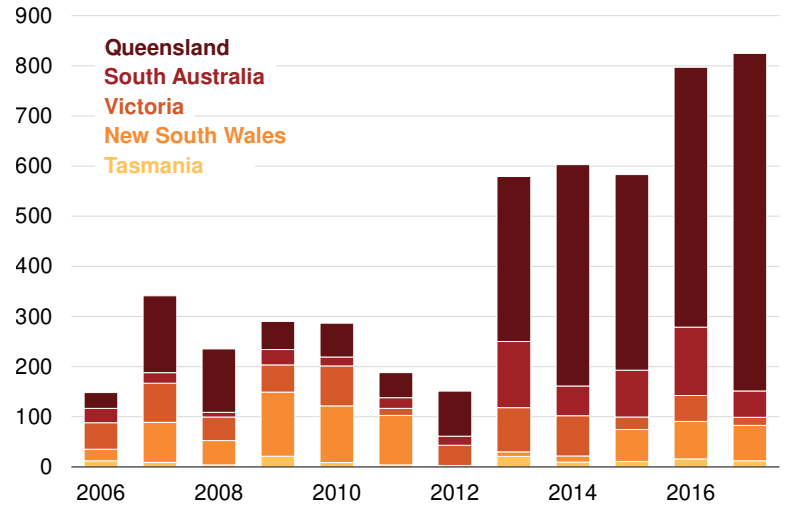
\includegraphics[width=0.6\textwidth]{Pictures/Chapter3/generator_gaming.png}
    \end{center}
    \caption{Increase in total value traded in the NEM from bidding games, \$ millions (Grattan Institute, 2018)}
    \label{fig:generator_gaming}
\end{wrapfigure}
Figure \ref{fig:wang_plot_full} highlights a number of key findings. Firstly. Since 2014, the arbitrage value of battery energy storage has clearly increased. 
\newline
Secondly, 2016 witnessed the highest revenues,  especially in South Australia.  \parencite{2016_prices} described the driving force behind the high volatility in 2016 attributable to the removal of the Northern Power Station. \textcite{2016_prices} also highlights a combination of high winter demand, low wind generation, planned upgrades to the Heywood interconnector, in combination with low levels of gas fired generation that coincided with high gas prices all contributed to high volatility.
\newline
Thirdly, Queensland in 2017 exhibited the highest revenue across the states. \parencite{grattan} attributes such volatility in 2017 to Queensland’s government-owned generation companies, Stanwell Corporation and CS Energy, (who provided 71 per cent of all electricity in Queensland in 2016–17), and reported record profitability; 30.4 and 58.9 per cent ROE, respectively. As shown in Figure \ref{fig:generator_gaming}, the value of bidding games have drastically increased in Queensland over the past decade. Gaming in the NEM can cause extreme price fluctuations, as shown in Figure \ref{fig:generator_gaming_1}. Figure \ref{fig:generator_gaming_1} highlights seven dispatch intervals that were near the market price cap of \$14,200/MWh, while most dispatch intervals were around \$100/MWh. In June 2017, the Queensland Government announced
the Powering Queensland Plan, which included a directive to Stanwell Corporation to \textit{“undertake strategies to place downward pressure on
wholesale prices"}. This aligns with Figure \ref{fig:wang_plot_full} as QLD 2018 revenues drop below NSW for the first time since 2011.
\begin{figure}
    \centering
    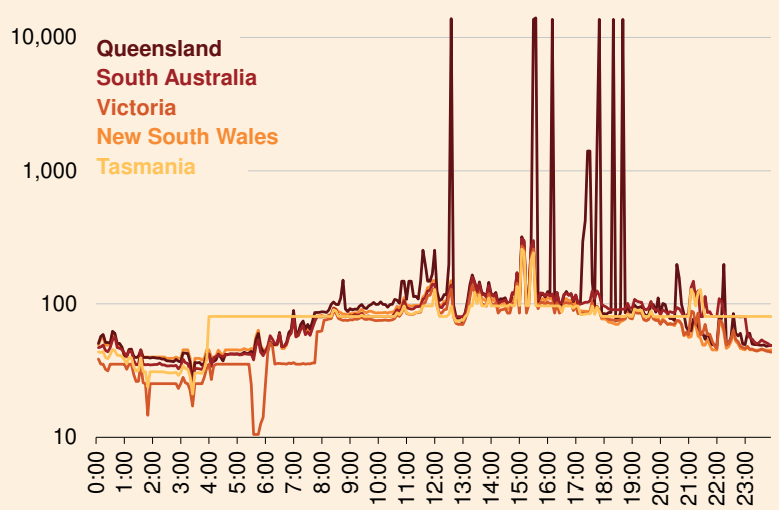
\includegraphics[width=0.6\textwidth]{Pictures/Chapter3/generator_gaming_2.png}
    \caption{5-minute dispatch interval
price by state for 12 January 2017 (Wood, 2018)}
    \label{fig:generator_gaming_1}
\end{figure}